%%%%%%%%%%%%%%%%%%%%%%%%%%%%%%%%%%%%%%%%%%%%%%%%%%%%%%%%
%
% UCF Electronic Dissertation and Thesis (ETD) Template
% (C) Copyright 2007-2014 Daniel Gallagher,
%
% https://bitbucket.org/dgallagher/ucf-thesis-latex-template
%
% Example chapter file
%
% Note:
%  - Chapter Titles must be ALL CAPS per UCF
%
%%%%%%%%%%%%%%%%%%%%%%%%%%%%%%%%%%%%%%%%%%%%%%%%%%%%%%%%

\chapter{FIRST CHAPTER} % Chapter titles in all caps per UCF Editor

\section{First Section}
\lipsum[2-3] % Placeholder text.

\section{Second Section}
\lipsum[4] % Placeholder text.

An example TikZ drawing is included in Figure \ref{fig:example}. Images can also be included as jpeg or png files using pdf\LaTeX. An example equation is shown in Equation \ref{eqn:example} and an example table is shown in Table \ref{tbl:example}.

\lipsum[5]

\begin{figure}
  \centering
  % Requires \usepackage{graphicx}
  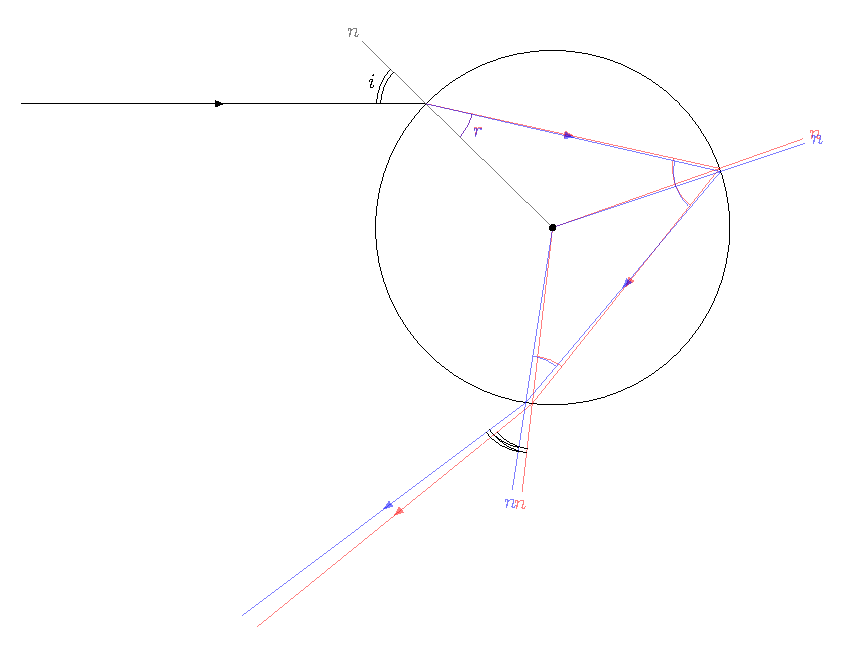
\includegraphics[width=\imsize]{figures/raindrop}\\
  \caption{Sun ray entering a rain drop}\label{fig:example}
\end{figure}

\lipsum[6]

\begin{table}
 \centering
\begin{tabular}{|l|c|p{3.5in}|}
\hline
\multicolumn{3}{|c|}{Places to Go Backpacking}\\ \hline
Name        &Driving Time   &Notes\\ \hline
Big Basin   &1.5            &Very nice overnight to Berry Creek Falls from either Headquarters or ocean side.\\ \hline
Sunol       &1              &Technicolor green in the spring. Watch out for the cows.\\ \hline
Henry Coe   &1.5            &Large wilderness nearby suitable for multi-day treks.\\ \hline
\end{tabular}
\caption{An example table.}\label{tbl:example}
\end{table}

\subsection{First Subsection}
\lipsum[7]

\begin{equation}\label{eqn:example}
x = \frac {-b \pm \sqrt {b^2 - 4ac}}{2a}
\end{equation}

\subsection{Second Subsection}
\lipsum[8] 